\documentclass[12pt, preprint]{aastex}
\usepackage{graphicx}
\usepackage{rotating}
\usepackage{amsfonts,amssymb,amsmath,mathbbol} 
\newcommand{\sersic}{S\'{e}rsic }
\newcommand{\iband}{$i$-band }


\begin{document}
\begin{titlepage}

\newcommand{\HRule}{\rule{\linewidth}{0.5mm}} % Defines a new command for the horizontal lines, change thickness here

\center % Center everything on the page
 
%----------------------------------------------------------------------------------------
%   HEADING SECTIONS
%----------------------------------------------------------------------------------------

\textsc{\LARGE Durham University}\\[1cm] % Name of your university/college
\textsc{\Large Physics Department}\\[0.5cm] % Major heading such as course name
\textsc{\large MPhys F301}\\[0.5cm] % Major heading such as course name

%----------------------------------------------------------------------------------------
%   TITLE SECTION
%----------------------------------------------------------------------------------------

\HRule \\[0.4cm]
{ \huge \bfseries Outer Profiles of S0 Galaxies in the Coma Cluster}\\[0.4cm] % Title of your document
\HRule \\[1.5cm]
 
%----------------------------------------------------------------------------------------
%   AUTHOR SECTION
%----------------------------------------------------------------------------------------

\begin{minipage}{0.4\textwidth}
\begin{flushleft} \large
\emph{Author:}\\
Shaun \textsc{Read} % Your name
\end{flushleft}
\end{minipage}
~
\begin{minipage}{0.4\textwidth}
\begin{flushright} \large
\emph{Supervisor:} \\
Dr. John \textsc{Lucey\\} % Supervisor's Name
\end{flushright}
\end{minipage}\\[1cm]



% If you don't want a supervisor, uncomment the two lines below and remove the section above
%\Large \emph{Author:}\\
%John \textsc{Smith}\\[3cm] % Your name

%----------------------------------------------------------------------------------------
%   DATE SECTION
%----------------------------------------------------------------------------------------

{\emph{Submitted: }\large{30 April 2014}}\\[1cm] % Date, change the \today to a set date if you want to be precise

%----------------------------------------------------------------------------------------
%   LOGO SECTION
%----------------------------------------------------------------------------------------
\begin{centering}
	\makebox[0.5\columnwidth]{
\includegraphics[width=0.5\columnwidth]{figs/Durham-University-Logo.png}}
\end{centering}

 
%----------------------------------------------------------------------------------------

\vfill % Fill the rest of the page with whitespace

\end{titlepage}


\begin{abstract}
	% !TEX root = master.tex

This study uses \iband imagery from both the Tenth Data Release of the Sloan Digital Sky Survey (SDSS DR10) and the latest MegaCam release to study truncated lenticular (S0) galaxies in the Coma cluster. Using an image from each camera we take two 1D profiles along the major axis of each. We develop algorithms for measuring sky, finding the break point and characterising the truncation for use with the 1D profiles. Using a sample of known disk galaxies, we refine the sample to include only 66 S0s with disk dominated outer disks. We find that $74^{+5}_{-5}\%$ of S0s are anti-truncated and $24^{6}_{-5}\%$ exhibit a pure exponential. Comparing to previous work in the Virgo cluster. We agree that there is a negligible fraction of truncated/down-bended disks in the cluster environment. We observe truncated

\end{abstract}
\maketitle
\tableofcontents

\section{Introduction}
	% !TEX root = master.tex
Ever since the 1920 Great Debate on the nature of nebulae, it has been known that the Milky Way is not the entirety of our universe, that there are indeed other `island universes' called galaxies \citep{berendzen_man_1976}. 

Modern ideas on how these immense structures formed describe quantum fluctuations in the very early universe becoming stretched during the inflationary period \citep{liddle_introduction_2003}. Significant gravitational perturbations arise out of these expanded wrinkles in space and after some time enough matter is accumulated and star formation can begin \citep{coles_cosmology:_2002}.

It is therefore important to understand the nature of galaxy formation if we wish to test cosmological models, since there is a direct relationship between large scale structure formation and cosmological parameters.

The most popular cosmology currently in use, $\Lambda$CDM (Cold Dark Matter), correctly predicts the existence of the CMB, the distribution of galaxies and the abundances of light elements \citep{liddle_introduction_2003} >>better reference<<. However, $\Lambda$CDM simulations diverge from observation at the galactic scale, predicting excessive numbers of dwarf galaxies \citep{silk_massive-black-hole-velocity-dispersion_2010} and too few massive bulgeless galaxies with thin disks \citep{kormendy_bulgeless_2010}.

Constraining galaxy properties with observation allows one to constrain or perhaps modify aspects of the $\lambda$CDM and hence lead to a more certain understanding of the early universe. >>More specifics<<

\subsection{Galaxy Properties}
Galaxies are not all indistinct clumps of stars but can take on a range of diverse structures \citep{hubble_no._1926}. Most galaxies can be crudely classified into three broad categories based on stellar content and morphology: Elliptical, Spiral and Irregular. 

Ellipticals are centrally condensed objects with a typical diameter from under 1 kpc to 200 kpc \citep{carroll_introduction_2007} and a smooth almost featureless luminosity profile. Ellipticals, as their name suggests, exhibit an elliptical shape range from ellipticity $\epsilon = 1$ (spheroidal E0) to around $\epsilon = 0.7$ (very oblate E7). 
Ellipticals contain little gas and hence little ongoing star formation due to their low gravitational binding energy \citep{crocker_molecular_2011}. 
Because they contain mostly old stars, ellipticals have higher metallicity and have moved off onto the red sequence, hence they are commonly called `red and dead' \citep{binney_galactic_1998}.  

\begin{figure}
	\label{galaxy type pictures}
\end{figure}

Spirals, in contrast, are very different to ellipticals in their structure. They are blueish disk galaxies usually with a redder central bulge and spiral arms with vivid dust lanes \citep{sparke_galaxies_2000}. The spiral arms are in fact density perturbations travelling around the disk, where the the increase in gas density initiates local star formation \citep{kennicutt_star_1998}. They therefore contain many more younger  main sequence stars, typically giving spirals a bluer hue of $0.4\lesssim B-V \lesssim 0.8$, where $B$ and $V$ are the magnitudes in the `blue' and `visible' wavebands in the UBV photometric system \citep{sparke_galaxies_2000}.

\subsection{S0s and Classification}
The traditional method of classifying galaxies is the Hubble Tuning Fork \citep{hubble_no._1926}. Hubble arranged galaxies from `early' to `late' types with the implicit assumption that all galaxies evolved that way in time. We now know that this transformation from early to late type is impossible since there is no way for ellipticals to increase their negligible angular velocity to match that of fast rotating spirals \citep{carroll_introduction_2007}. 

Spirals are sorted by the bulge size and tightness of their spiral arms and ellipticals by their ellipticity. On this continuous fork, an intermediate `lenticular' class is necessarily created. 
\begin{figure}
	\label{hubble_fork}
\end{figure}
Lenticulars, or S0 galaxies, are observed to share the stellar content of ellipticals but the structure and kinematics of spirals. They are disk galaxies but have a smooth brightness profile free from spiral arms \citep{blanton_physical_2009}. S0s can be dusty and have few HII regions associated with young stars \citep{degraaff_galaxy_2007}. Together with a high metallicity, these properties give the galaxy a `red and dead' appearance with $0.7\lesssim B-V \lesssim 0.9$.

Due to their similarity with ellipticals, there have been many misclassifications of S0s with low inclinations (side-on) \citep{laurikainen_multicomponent_2005}. 
S0s do not have significant emission on the H$\alpha$ line and estimates of dynamical mass become challenging \citep{dressler_rotational_1983}. S0s have a central spheroidal component or bulge, which on average, is flatter than an elliptical and usually brighter than its disk unlike spiral bulges \citep{dressler_galaxy_1980}.

\subsection{Photometry}
Morphological classification remains, by its qualitative nature, subjective and open to interpretation \citep{naim_automated_1995}. Using the quantitative measure of galaxy luminosity profiling minimises disagreement between observers and helps to quantify physical properties with more certainty. 

Profiles are generated by isophotal analysis, whereby one fits thin ellipses of equal intensity (an `isophote') to the image, working outwards from the previously established centroid. Plotting the average isophote intensity against geometric mean radius to generate a 1D intensity profile \citep{peng_detailed_2002}. Now galaxy can be fitted by mathematical models and the resulting parameters analysed. 

De Vaucouleurs was one of the first to propose his $R^{1/4}$ model for galaxy light distribution \citep{de_vaucouleurs_revised_1963}. This model was successful in fitting elliptical galaxies and is still used today with bulges of S0 and spiral galaxies \citep{allen_millennium_2006}. However, this model does not describe all bulges well and an exponential model best describes disks! Given this variation in model parameters, the De Vaucouleurs model can be generalised to a \sersic $R^1/n$ model \citep{sersic_atlas_1968}.
\begin{equation}
		I(R) = I_{e} \rm{exp}\left\{-b_{n}\left[\left(\frac{R}{R_{e}}\right)^{1/n} - 1\right]\right\},
\end{equation}
where $I(R)$ is the intensity at radius $R$, $n$ is the Sersic index, $R_e$ is the effective radius which encloses half the total intensity, $I_e$ is the intensity at $R_e$ and $b_n$ is defined such that $\Gamma(2n) = 2\gamma(2n, b_n)$, where $\Gamma$ is the complete gamma function and $\gamma$ is the incomplete gamma function.
\begin{figure}[!ht]
		\centering
		% 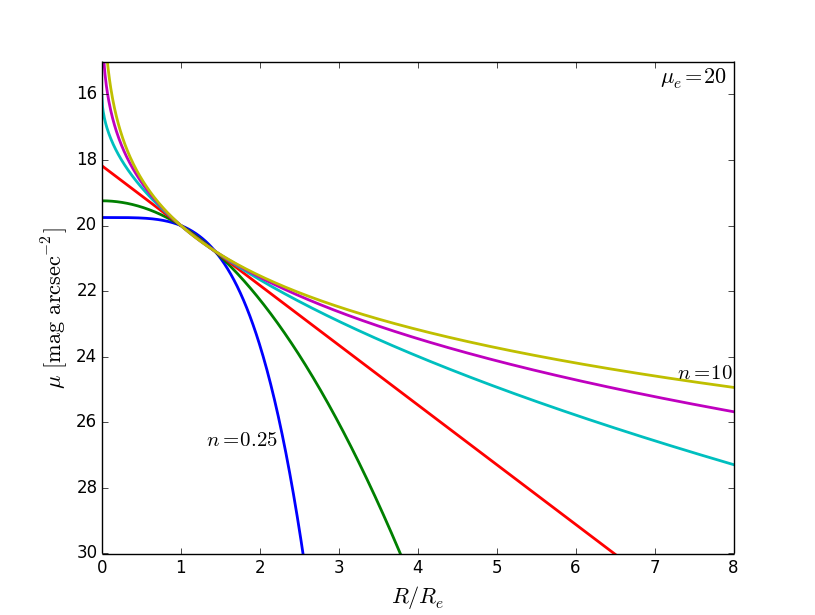
\includegraphics[width=\linewidth]{sersic_mags}
		\caption{Magnitude profiles of Sersic indices from 0.25 to 10}
		\label{fig:sersic_mags}
	\end{figure}
\ref{fig:sersic_mags} shows the effects of adjusting the \sersic index with respect to a constant effective surface brightness. As $n$ becomes smaller, the light becomes less centrally concentrated and lower in central intensity \citep{graham_concise_2005}. 

Most galaxies do not consist purely of one component \citep{laurikainen_multicomponent_2005}, but include several, such as disks, bulges and bars. The \sersic model has been found to fit all of these components with low residuals and is reliably used to classify galaxies into morphological type \citep{peng_detailed_2010}.

\subsection{The origins of S0 Galaxies}
The origin of lenticular galaxies remains a highly active area of research. Logic dictates two possibilities for S0 formation: Either they formed in the same manner as ellipticals at the start of the galaxy formation era or they have since evolved from spirals by some unknown mechanism \citep{burstein_k-band_2005}.

If S0s did indeed transform from spiral-like galaxies, then a corresponding increase in the population of spirals should be seen over increasing redshift. This trend has been observed, showing an increase in early-types with look-back time \citep{dressler_evolution_1997}.

There is also evidence from Tully-Fisher Relation (TFR), in which galaxy luminosity is related to maximum rotational velocity \citep{tully_new_1977}. This relation is tightly defined for local spirals, with a small intrinsic scatter, as $0.43 \pm 0.03$ mag averaged over SDSS griz bands \citep{pizagno_tully-fisher_2007}. Now that reliable TFRs have been constructed or S0s \citep{bedregal_tullyfisher_2006}, the existence of an offset from spirals is confirmed. S0s are fainter than spirals by an average of $0.85 \pm 0.19$ mag in the $i$-band, with a similar offset is found in the $g$ and $K_s$ bands \citep{rawle_s0_2013}. This offset can be interpreted as the cessation of star formation and subsequent fading of the disk.

Various mechanisms for quenching star formation have been proposed. Ram-pressure stripping removes the disk gas necessary for subsequent star formation \citep{gunn_infall_1972}; strangulation would remove larger reservoir of halo gas, having a slower and gentler impact on star formation; or the harsher minor merger of two spirals, exhausting a large amount of the interstellar medium (ISM)  \citep{bekki_unequal-mass_1998} to name but a few.

Given that the typical surface brightness of S0s has actually found to be greater than that of spirals \citep{burstein_k-band_2005}, this suggests that the bulge luminosity of S0s is too large to evolve from disk fading alone \citep{cortesi_planetary_2013}. The increased brightness favours minor mergers or galaxy harassment, where frequent high speed encounters strip disk gas and dump some of it at the centre \citep{moore_galaxy_1996}.

The well-known morphology-density relation \citep{dressler_galaxy_1980}, describes an increase in early types with projected surface density. This is to be expected if S0s result from galaxy interactions but S0s are observed in the field, suggesting that this may not be the whole story. If this is indeed the case, then either cluster based mechanisms such as ram-pressure stripping cannot be responsible for S0 formation, or there are multiple evolutionary paths to S0s operating in different environments. 

If the evolutionary mechanism is dependent on density, then there might be structural differences in S0 galaxies as a function of environment which can be used to probe evolutionary history.
>>>see head for good description of fading process<<<

\subsection{Truncation}
-infinite exp. doesn't describe completely, most disks
-three classes of truncation
-graphs of own truncated gals
-erwin



One feature, suitably sensitive to external interactions, is the outer structure of the disk \citep{pohlen_stellar_2004}. The outermost radii should be vulnerable to the effects of galaxy-galaxy interactions, late-time accretion and gas stripping, hence retaining an imprint of formation process. 

Disk galaxies have been known not to obey an infinitely extended exponential light distribution for 35 years \citep{van_der_kruit_optical_1979}. It has become apparent that most (79\% according to \citet{pohlen_cut-off_2001}) disk galaxies exhibit `truncations' or `breaks' in their otherwise smooth exponential profiles. 

S0 galaxy truncations can fall into three broad truncation classes: Type-I: single-exponential, Type-II: classicly truncated \citep{freeman_disks_1970} or Type-III: anti-truncated \citep{erwin_antitruncation_2005}. 
\begin{figure}
	\label{own sample examples on truncated types}
\end{figure}

Though early analysis indicated an even distribution of types in local S0s \citep{gutierrez_outer_2011}, when the cluster and field are analysed separately a distinct difference arises. While field S0s are divided roughly evenly between all three types, Virgo S0s appear to be completely devoid of type-IIs with $M_v < -17$ $f_{S0} = 0_{-0}^{+4}\%$ \citep{erwin_strong_2012}. Since type-IIIs are found to be equally common in both environments, the difference is made up of type-I profiles, making single-exponentials twice as common in the Virgo cluster than in the field. 

To account for such a drastic change in type population, either something in the (early) cluster transforms type-II into type-I or something prevents the opposite transition which is common in the field. Assuming cluster S0s originally had type-II truncated profiles, then a mechanism is required which erases said truncation. Harassment is a popular take ............

\subsection{Aims of Project}
- is it possible to find and classify truncations using a 1D profile method
-compare and contrast Virgo and Coma
-variation within the cluster
-search for a correlation between \sersic parameters and trunc. type

In this project, we investigate the feasibility of detecting and classifying truncations in the coma cluster S0s using a simple 1D bulge-disc decomposition procedure. 

\citet{erwin_strong_2012} used a sample of 24 S0s within the Virgo cluster. By studying Coma S0s we can select a larger number of S0s over a wide range of cluster-centric radii and hence compare and contrast the results with \citet{erwin_strong_2012}. 

In addition, we also investigate truncation type as a function of cluster-centric radius in an effort to see if the truncation mechanism also depends on cluster density as well as cluster membership.

Lastly, a search for a correlation between \sersic parameters and truncation type is investigated.


\section{Data and Initial Sample}
	% !TEX root = master.tex
An initial large sample of 620 galaxies of disk galaxies from \citet{head_dissecting_2014} in the Coma Cluster was used as a basis for further refinement. Cluster membership was determined by a redshift of $~0.023$ with the centre of Coma taken as the mid-point between NGC4874 and NGC4889.

The \iband was selected in order to avoid the catastrophic OH-brightening and water absorption in the far-infrared and to enhance detection of `red and dead' S0s. Images were obtained from both SDSS and MegaCam for each galaxy in the sample. A point spread function (PSF) full-width half-maximum (FWHM) of between $0.65''$ and $0.84''$ was typical \citep{head_dissecting_2014}. The pixel scale was $~0.396$ arcsec pix$^{-1}$ for SDSS and $~0.186$ arcsec pix$^{-1}$ for MegaCam. 
\section{Data Reduction and Analysis}
	% !TEX root = master.tex
\subsection{Extracting 1D profiles}
We extract two 1-dimensional profiles for each image. In our implementation, wedges drawn along each direction of the major axis centred by fitted isophote ellipses and the median counts are calculated along the axis at regular intervals (with central counts being determined by interpolation). The profile is terminated when the counts become consistently lower than the sky value given by SDSS/MegaCam pipeline. This results in four 1D profiles for each galaxy with varying sizes of regions where the sky becomes dominant. 

\subsection{Sky subtraction}
\subsubsection{The effects of sky}
The night sky is never completely dark and in the \iband it has a brightness of $19.9$ mag $\rm{arcsec}^{-2}$ \citep{binney_galactic_1998}. Indeed, proficient sky subtraction is required for the acquisition of accurate surface brightness profiles at low brightness. If the sky background is underestimated, the sky will contribute to the profile at large galactic radius and flatten off the profile if sufficiently extended. If the background is overestimated, light from the galaxy is subtracted also, plunging it towards zero at some finite radius. 
\begin{figure}
	\label{fig: effects of sky from binney}
\end{figure}
There are, however, other errors that contribute to the overall corruption of the image besides sky estimation. Due to the limitations of optical devices and CCDs, there may be a gradient across an image frame to due to CCD bias or inhomogeneous illumination \citep{olsen_radiometric_2010}. Joining frames together, or `splicing' exacerbate this effect since different exposures will have different sky backgrounds. The raw data is already corrected for this by SDSS and MegaCam in flat-fielding corrections, but the correction is not perfect and may result in unwanted artefacts or gradients across the image. SDSS operates in drift scan mode \citep{abazajian_seventh_2009} and so does not suffer as much from the effects of flat-fielding since any bias or aberration is averaged out.

\subsubsection{Finding the sky}
Accurate background estimates are essential in characterising outer profiles. While both cameras give their own estimated sky fluxes and the extraction of 1D profiles yields a additional estimate, background can vary within images -and therefore, between major axis profiles- due to flat-fielding errors \citep{bijaoui_sky_1980}. We have found that our estimate of the sky differs by as much as $4.9$ counts from the SDSS/MegaCam sky value.

\begin{figure}
	\caption{Flow chart of the sky finder}
	\label{fig: }
\end{figure}

To find the radial position at which the sky starts to dominate, the profile is divided into chunks of three data points. For each chunk, the local mean and standard deviation are calculated. This is essentially finding the local value of intensity. We define the point at which the sky starts to dominate as the point where $\bar{I}_{i+1} > \bar{I}_i + \sigma_i$, where $\bar{I}_i$ is the local mean intensity and $\sigma_i$ is the standard deviation at point $i$. We initiate this search from the end of the profile. The effects of local minima and maxima due to stars and noise are also taken into account by considering the next two local means instead of just one (i.e. $\bar{I}_{i+2}$).

\begin{figure}
	\caption{Depiction of sky area}
\end{figure}

The mode is the best estimate for the sky value since it is the peak of the brightness frequency distribution \citep{bijaoui_sky_1980}. Therefore, we use a $3\sigma$-clipped, synthetic mode to estimate the sky values.

The value for sky uncertainty is calculated by first `clipping' the sky dominated area so that values that lie further than $3\sigma$ away from the mean sky value are removed. We use a similar synthetic mode to \citet{peng_detailed_2010} of $3(\rm{median}) - 2(\rm{mean})$ to calculate sky brightness along with its standard deviation for the sky uncertainty.

We define the critical surface brightness $\mu_{crit}$ as the surface brightness up to which the profile is considered reliable. $\mu_{crit}$ is placed where we calculate the difference between under and over subtracted profiles (i.e. $\pm 1 \sigma_{sky}$) to be 0.2 mag. This is a more useful measurement of sky than a $\pm 3 \sigma$ since it shows us where the actual profile starts to be affected.

\subsection{Bulge-Disc decomposition}
\sersic parameters for each profile are determined by bulge-disc decomposition. We use the Levenberg-Marquardt non-linear least squares regression algorithm (LMA) to minimise chi-squared and fit the profile to the desired model. Reduced chi-squared is used as a goodness-of-fit measure.
\begin{equation}
	\chi^{2}_{\nu} = \frac{1}{N-n-1} \sum_{i} \frac{[y_i - f(x_i)]^2}{w_i^2},
\end{equation}
where $\chi_{\nu}^2$ is the reduced chi-squared goodness-of-fit measure, $N$ is the number of data points, $n$ is the number of free parameters, $y_i$ are the data points, $f(x_i)$ are the associated model points and $w_i$ are the associated weightings for each point \citep{marquardt_algorithm_1963}. A reduced chi-squared of $\chi_{\nu}^2 \approx 1$ describes an accurate fit, $\chi_{\nu}^2<1$ describes overestimated errors and $\chi_{\nu}^2>1$ is degenerate in describing both underestimated errors or an incorrect model. This is by far the most tested and reliable fitting method \citep{lawson_solving_1995} and was implemented in the high-level language Python with Scipy \citep{oliphant_python_2007}. 

We use an exponential disk + \sersic $R^{1/n}$ bulge model used in \citet{allen_millennium_2006} as bulges cannot all be described by $R^{1/4}$ \citep{simard_catalog_2011}. Fitting a model with six parameters is challenging to accomplish in one fell swoop since there is more parameter space to explore and so the likelihood of being trapped in a local minima -and not a global minima- increase. Therefore, we employ an iterative method similar to that found in \citet{weinzirl_bulge_2009} as follows:

\begin{enumerate}
	\item \sersic fit: \\
	A \sersic bulge (free $n_B$) is fit to the profile with a radial surface brightness of:
	\begin{equation}
		I(R) = I_{e} \rm{exp}\left\{-b_{n}\left[\left(\frac{R}{R_{e}}\right)^{1/n} - 1\right]\right\},
	\end{equation}
	where we use the definitions given earlier.	LMA converges quickly to a solution for a single \sersic roughly independent of initial parameter guesses. 

	\item Bulge+disk fit: \\
	The \sersic bulge is duplicated and has its \sersic index $n$ set to unity. The model now reads:
	\begin{equation}
		I(R) = I_0 \rm{exp}\left\{-\frac{R}{h}\right\} + I_{e} \rm{exp}\left\{-b_{n}\left[\left(\frac{R}{R_{e}}\right)^{1/n} - 1\right]\right\},
	\end{equation}
	where we now use the scale length $h=R_{e,D}/1.678$ and central intensity $I_0=I_{e,D}e^{-1.678}$ instead of $R_{e,D}$ and $I_{e,D}$ in order to distinguish concisely between bulge and disc parameters. 
\end{enumerate}

Fitting the usual assortment of effective magnitudes, effective radii and \sersic indices will sometimes result in an Allen Type-4 `inverted' profiles where the bulge dominates at large radii and the disk dominates at the centre \citep{allen_millennium_2006}. 

	Since we have already removed the sky and specified that we reject galaxies whose bulge dominates at large radii, we can assume that these solutions are likely the result of LMA attempting to fit a truncation or some other object such as a foreground star. To avoid these unreal solutions, the bulge+disk system is fit using effective radii and bulge-disk ratios (henceforth known as $\Delta R_e$ and $B/D$) instead of the parameters themselves. Limits are placed upon them such that $B/D < 1$ and $\Delta R_e = 1.678 h / R_e > 1$, to only permit disk dominated solutions. 

	\begin{equation}
		\frac{B}{D} = \frac{n \Gamma(2n)}{b^{2n}}\left(\frac{R_e}{h}\right)^{2} \left(\frac{I_e}{I_0}\right),
	\end{equation}
	where $b = b_{n,bulge}$.

Weights for use in LMA are computed in raw photon counts on a per pixel basis. The total error in intensity for each point is given by 
\begin{equation}
	\alpha = \frac{1}{s_{pix}^2}\sqrt{\alpha_I^2 + \alpha_{extraction}^2 + \alpha_{sky}^2},
\end{equation}

where $s_{pix}$ is the pixel scale, $\alpha_{extraction}$ is the error in forming a 1D profile along the major axis, $\alpha_{sky}$ is the sky uncertainty and $\alpha_I$ is the error in counts given by 
\begin{equation}
	\frac{\sqrt{I_{phot}G}}{G},
\end{equation}
where $I_{phot}$ is the raw photon count and $G$ is the CCD gain.

\begin{figure}
	\caption{Diagram showing differences between fitting in ratios and without}
\end{figure}

\subsection{Truncation detection}
% - fitting a BD is helpful (see results)
% - define a break
% - derive a break radius for each galaxy 
% - break region/uncertainty/smoothness
% - fitting the two truncations
% - assume only two breaks
Fitting a galaxy with an un-truncated model, as above, is helpful to quantify the bulge size. It even gives some measure of truncation type through its residuals (see results). 

To quantify a truncated surface brightness profile, three bulge parameters; two sets of scale lengths and central magnitudes; and a break radius are required. We do not fit a truncated model straight to the whole surface brightness profile as this is yet more unstable than the five parameter bulge-disc model due to the additional three parameters needed. We use a method similar to that of \citet{pohlen_structure_2006} whereby we instead, derive the break radius and then fit two separate profiles to the disk dominated area.

We define a disk dominated region where the disk is not more than 0.2 mag away from the total surface brightness and is not smaller than $\mu_{crit}$. This avoids noise from both the sky and the bulge.

The new disk profile is first smoothing using an unweighted B-spline function \citep{dierckx_curve_1975} of order 3. Then a median-filter is used to remove the last of extreme values with a smoothing length of 10\% of the length of the region.
The profile is then broken into overlapping chunks of three data points, to which a straight line is fitted. This results in an approximated derivative of the profile and estimate of the local scale length $h_{loc}$ at each point. 

\begin{figure}
	\caption{truncation break radius derivation graph}
\end{figure}

Since the transition from scale lengths at the break radius has been found to be frequently smooth \citep{erwin_outer_2008,pohlen_stellar_2004,maltby_anti-truncated_2011}, we assume that there are now two regions of constant scale length joined by a transition region. 

We define the boundaries of the transition region as the point where the local scale length - starting from the break radius - reaches a value of $1\sigma$ away from the inner and outer means. These boundaries provide a measure for break radius uncertainty. 

We then proceed to fit a straight line to the magnitudes of both the inner and outer disk regions. We do not use the intensity counts because the outer disk is usually plagued with negative values and it is less computationally intensive. Due to fact that the break region may be large, we do not restrict ourselves to not fitting inside it.

Classification of three or more such breaks is not uncommon in other works \citep{pohlen_structure_2006,gutierrez_outer_2011} but does lead to complications when trying to find the means around each break radius. In our investigation, it is assumed that there are no more than two break radii and this works well for the majority of cases. 

\subsection{Parameter uncertainties}
The uncertainties of LMA can be computed from the covariance matrix of a fit \citep{hughes_measurements_2010}, but we implement a bootstrapping resampling procedure to estimate the errors on each fit parameter. 

We resample our data points, with replacement, and fit 3000 times to get a distribution for each parameter. The standard deviations and means are then calculated from this distribution.

In addition to the errors due to sampling and fitting (measured by bootstrapping), we calculate the error due to sky uncertainty. The profile is raised and lowered by the sky uncertainty and is refit with these new values of intensity. 
\section{Results}
	% !TEX root = master.tex

% talk about initial disk fitting- disk dominated section, fit without weights etc

% Fitting a galaxy with no truncations as above, is helpful to quantify the bulge size. It also provides a reliable, if not robust, measure of truncation type through its residuals. - tighter weighting results in a good measure for truncation type further out

\subsection{Sky Detection} % (fold)
\label{sub:sky_detection}
The automated detection routine as describe above successfully finds the sky dominated area with all sample light profiles. The sky value obtained from our detection algorithm differed from the values delivered from the SDSS/MegaCam pipeline by as much as 5\%, though typically only differs by about 0.3\%.  Sky uncertainty as the standard deviation differs from the pipeline uncertainties ($\sqrt{sky}$) by around 40\%. 
\begin{figure}[h]
	\centering
	\makebox[0.7\columnwidth]{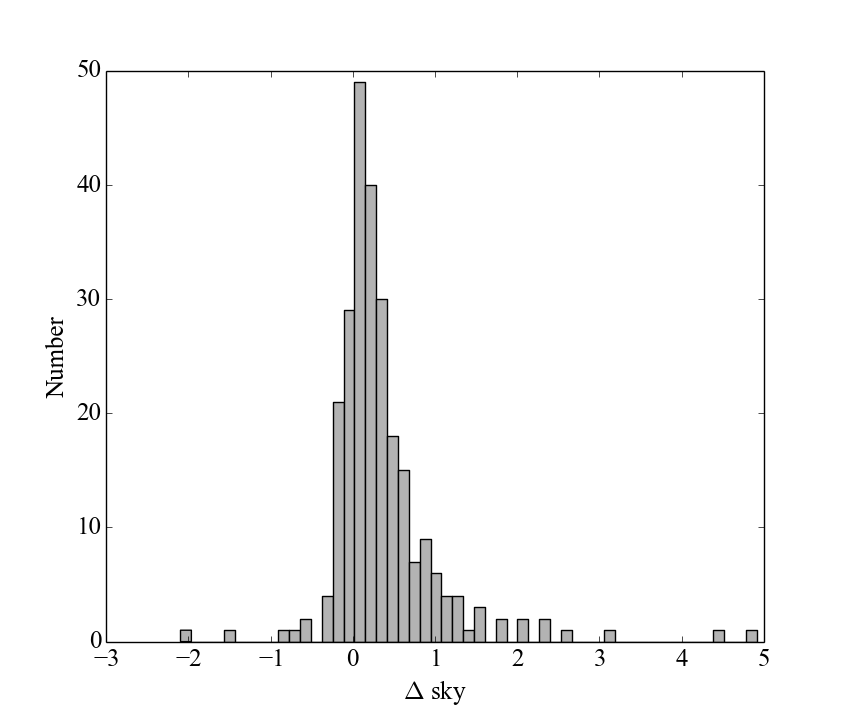
\includegraphics[width=0.7\textwidth]{figs/sky_hist.png}}
	\caption{\footnotesize{Histogram of the differences between our sky values and MegaCam/SDSS}}
\end{figure}

% subsection sky_detection (end)


\subsection{Example Decomposition} % (fold)
\label{sub:example_decompositions}
We present a typical galaxy decomposition and classifications for a disk exhibiting upbending to illustrate the classification process. ID 1237667444048265310 is a typical example of a type-III classified galaxy.

\begin{sidewaysfigure}[p]
	\centering
	\makebox[1.\columnwidth]{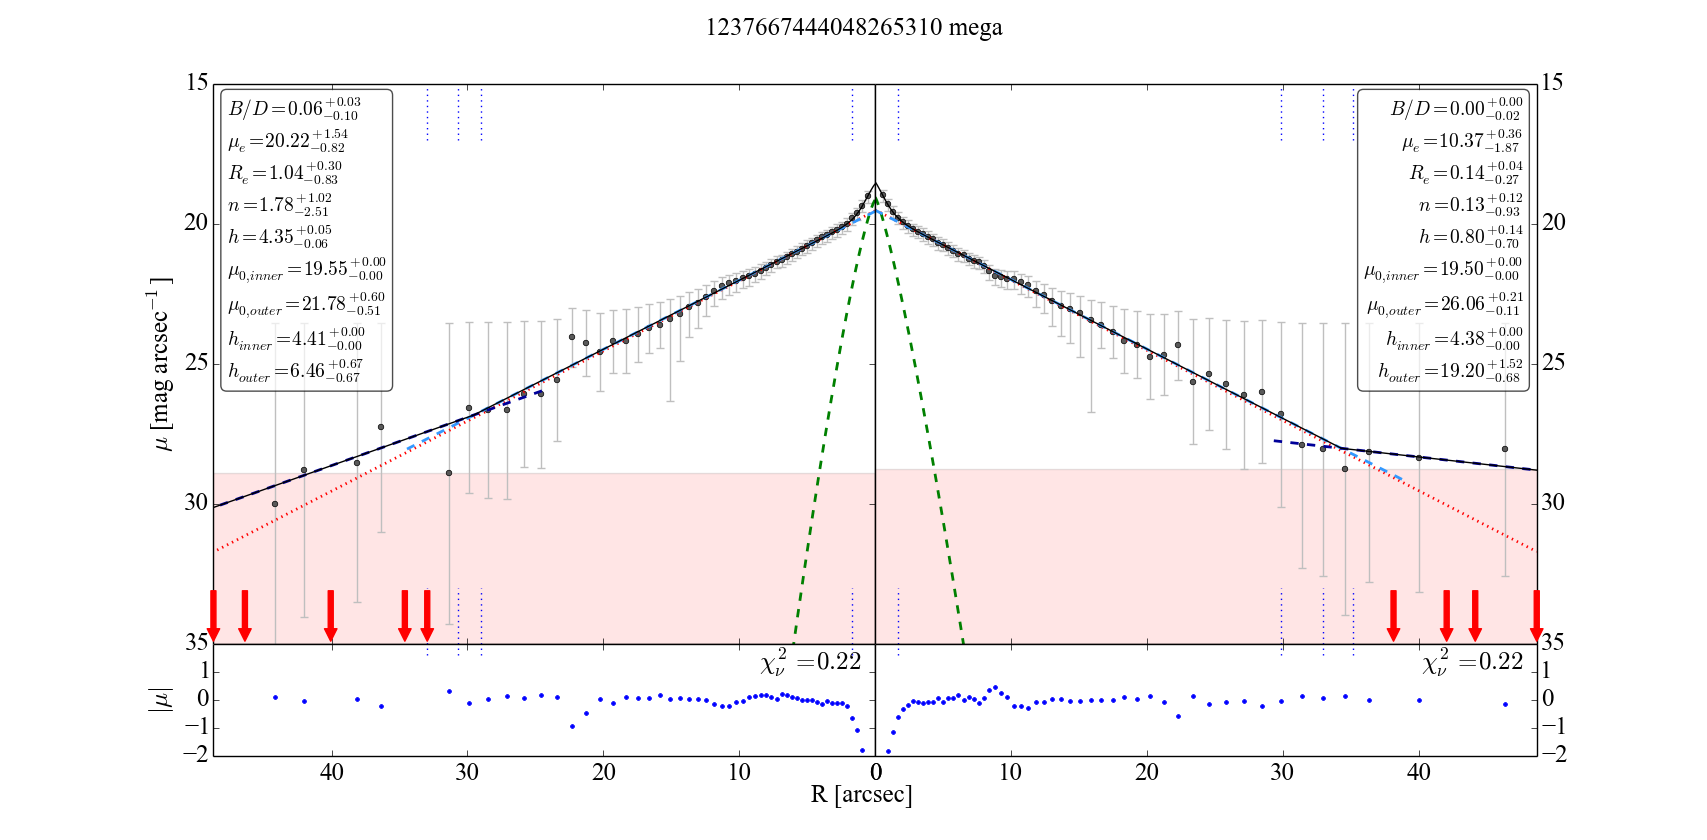
\includegraphics[width=1.5\textwidth]{figs/example_decomp.png}}
	\label{fig: The mega profiles of 1237667444048265310}
	\caption{\footnotesize{The surface brightness profile for the MegaCam image of 1237667444048265310. The plot shows the inner and outer disks in light and dark dashed lines respectively. The bulge is illustrated in green and the original pre-truncated disk is shown as a red dotted line. The total is depicted with a thin black line.
		 Unreal (negative counts) values are shown with red arrows and the critical sky value as the red region. The dashed lines at the top and bottom denote the lower sky limit, lower break limit, upper break limit and bulge cut-off radius, working inwards. Normalised magnitude residuals are shown at the bottom.}}
\end{sidewaysfigure}
Figure \ref{fig: The mega profiles of 1237667444048265310} shows the surface brightness profile of 1237667444048265310. Both MegaCam profiles, representing the different major axes, are completely independently fit. This galaxy is a typical example of an error in truncation detection. Usually there is one profile per galaxy which exhibits this undesirable behaviour. This problem cannot be remedied by restricting the parameters in the fit, since any more restriction tends to yield unreal solutions such as lack of bulge.

Firstly, a simple bulge + disc is fit to the profile, resulting in a typical profile with a disc scale length of $\sim 6$ arcsec and bulge effective surface brightness of $\sim 20$ mag. 

On the other hand, the bulge shape -characterised by the \sersic index- varies between SDSS and MegaCam fits. Though this changes the shape of the bulge entirely, its surface brightness remains small enough ($\mu_B < \mu_D + 0.2$ mag) as to not have an impact the total at large $R$.

Next, the automated truncation detection yields a potential break point and the two disks are parameterised. The routine classifies these individual fits as Type-III (upbended) since the lower limit on the outer scale length does not fall below the upper limit on the inner scale length. 

As seen in the residual plot accompanying the fits, there is poor fit at the centre of the galaxy, where the bulge is strongest. Since the truncation fit only subtracts the bulge's contribution to the total magnitude, it is likely that the poor central fit is due to neglection of bulge light.

The next step is to combine the images to yield overall parameters for the entire galaxy. However, although there is a good agreement of pre-truncated-fit -called `classic' from now on- disk parameters between cameras there is a discrepancy in the \sersic index of the bulge. SDSS fits a small $n\approx 0.5$ bulge whilst MegaCam finds an expansive $n\approx 1.5$ bulge. 

This discrepancy error is a major problem when combining results as averaging the parameters does not yield an accurate `one-size-fits-all' solution. The truncation is commonly classified differently between cameras. We proceed by combining their bootstraps instead. This does not solve the problem of not yielding an accurate solution but it does provide an accurate error on the result, unlike a weighted arithmetic mean \citep{andrae_error_2010}. 

Defining the truncation strength as 
\begin{equation}
	S_h =  \frac{h_{outer} - h_{inner}}{h_{inner}},
\end{equation}
we find that $S_h = 1.3^{+0.9}_{-0.7} > 0$ for the combined profile and so is classified as Type-III.

% subsection example_decompositions (end)

\subsection{Sample Properties}
\begin{sidewaysfigure}[ph]
	\makebox[1.\columnwidth]{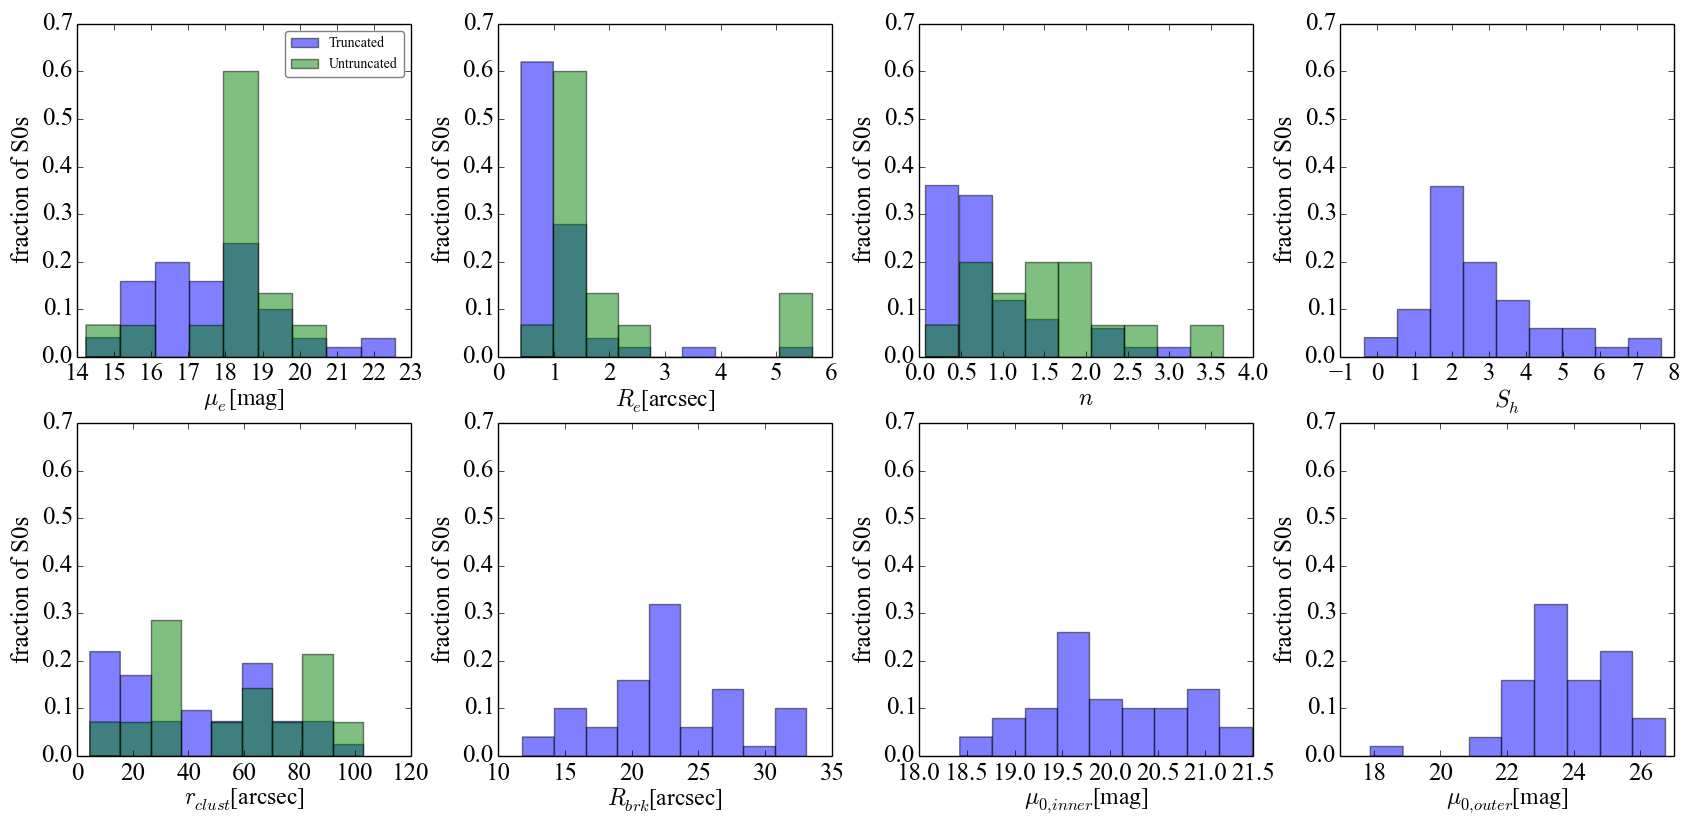
\includegraphics[width=1.\textwidth]{figs/props_hist.png}}
	\caption{\footnotesize{Proportion of both truncated and untruncated disks as a function of various parameters where available}}
	\label{fig: prop_hist}
\end{sidewaysfigure}
Though all profiles have been successfully fit with a disk dominated outer profile, it was not always real. There were frequent situations where a disc with perturbation (Allen type-6) were fit. These galaxies usually had what appears to be previously unseen spiral patterns, wide bars or simply a bulge dominated outer profile. Since these components are not part of this investigation, these galaxies were discarded.

We restricted ourselves to using galaxies with inclination (axis ratio) $b/a > 0.4$ and bulge size $R_{e,bulge} < 0.2R_{e,disk}$. This removed a great many bulge dominated systems, shrinking our sample to 83 galaxies. The initial sample of profiles was also filtered by removing galaxies whose profiles yield hugely disagreeing results. This was done by eye and the sample was refined to 66 reasonable fits. 

Our sample exhibits a range of bulge sizes, showing that our restrictions on bulge parameters relative to the disk has had little impact on the diversity of our sample. With a typical bulge of $R_e = 1.0\pm 0.9$ arcsec and $n = 0.8\pm 0.7$, the bulge clearly tends to be less luminous that the disk in truncated systems and more centrally concentrated than in type-Is ($R_e = 2\pm 1$ arsec and $n = 1.5 \pm 0.9$). The type-III preference for a more centralised bulge suggests that the upbending is not due to bulge influence at large $R$, which earlier, may have escaped notice. 

In Type-III disks, the central surface brightness of the outer disk must be greater than that of the inner disk. This can clearly be seen in the sharp divide between the distributions in figure \ref{fig: prop_hist}. The typical inner central surface brightness is $20.0\pm 0.8$ mag whereas in the outer disk it spans a wider range of values with a higher mean $24 \pm 2$ mag.

In truncated galaxies, the break point takes a wide range of radii and the strength of the break exhibits a peak at 2. The small number of truncated galaxies with low break strength can be attributed to the classification process, since a low break strength is more likely to lie within $\sim 1\sigma$ of the classical disk and hence classified as untruncated. 

\begin{figure}[h]
	\centering
	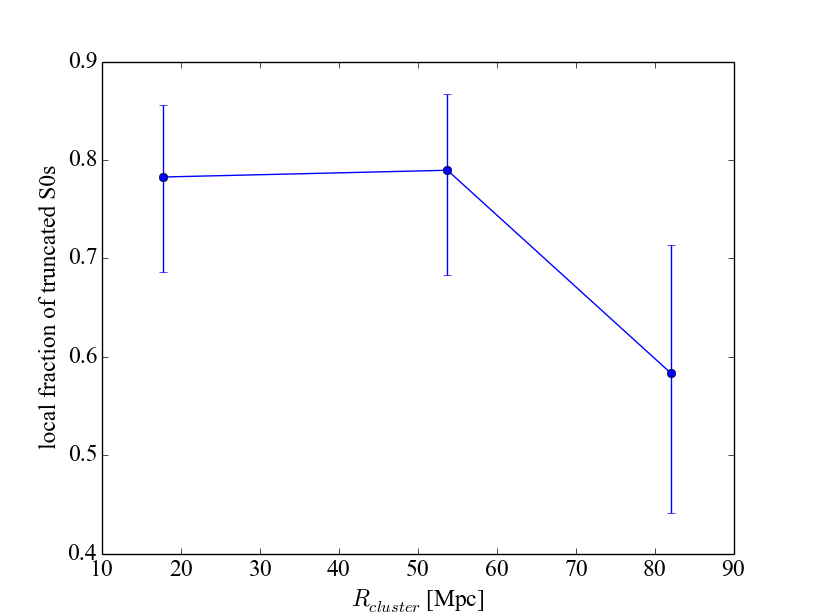
\includegraphics[scale=0.5]{figs/fraction_vs_cluster_radius}
	\caption{\footnotesize{Fraction of upbended S0s binned with equal distance bins. Error bars show 68\% confidence intervals \citep{wilson_probable_1927}}}
	\label{fraction vs dist}
\end{figure}

We find that  $74^{+5}_{-5}\%$ of S0s in the Coma cluster are anti-truncated type-IIIs and a corresponding $24^{+6}_{-5}\%$ are untruncated. The remaining 2\% of type-IIs consist of one galaxy (see Discussion for further information). 

% subsection Sample Properties (end)

\subsection{Correlations} % (fold)
\label{sub:correlations}
We found no statistically significant evidence of a trend between distance from cluster centre and bulge and classical disk parameters . However, there is a parabolic region of $30 \lesssim R_{clust} \lesssim 60$ arcsecs, $28 \lesssim \mu_{0,outer} \lesssim 25$ mag in which there are no truncated galaxies.

There is a slight trend for truncated galaxies to be found at lower cluster radii seen in figure \ref{fig: prop_hist} but this is not statistically significant.

We found evidence of a weak trend between the bulge magnitude and the break radius. A Pearson correlation coefficient of 0.26 indicates an increase in bulge magnitude as the break appears further out in $R$.
\begin{figure}[ht]
	\centering
	\label{bulge/break correlation}
	\makebox[0.8\columnwidth]{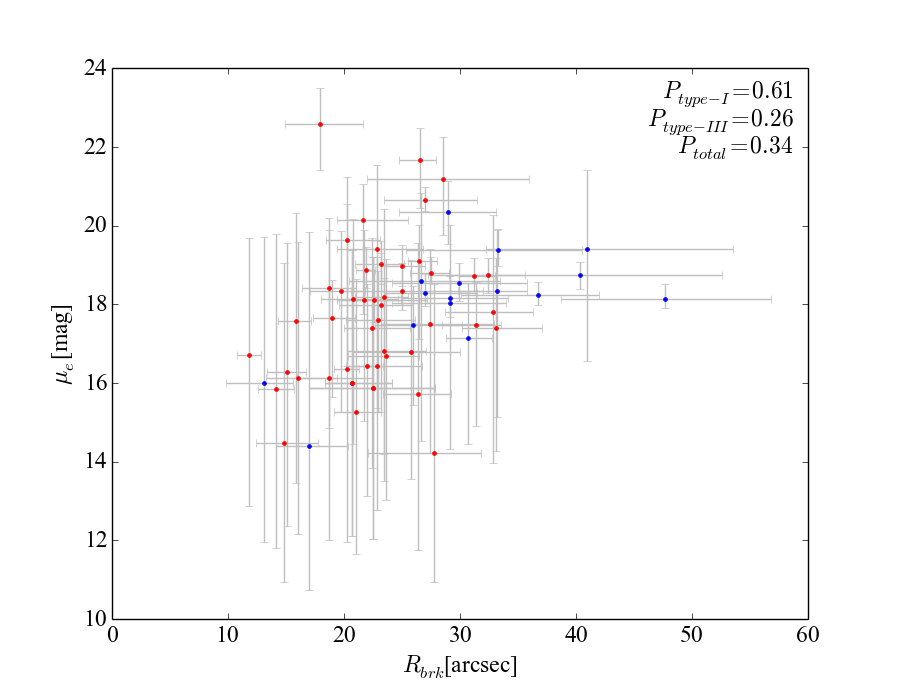
\includegraphics[width=0.8\textwidth]{figs/bulge_mag_vs_brk.png}}
	\caption{\footnotesize{A correlation plot between effective bulge magnitude $\mu_e$ and break radius $R_{brk}$ with truncated galaxies shown in red and untruncated galaxies shown in blue for comparison.}}
\end{figure}
Type-I S0s exhibit a tighter correlation between their potential break radius and bulge magnitude. This demonstrates that this trend is likely an artefact of the fitting process.

A weak trend in fraction of type-III against cluster-centric radius is observed when binning the galaxies into inner, outer and intermediate radii (see figure \ref{fraction vs dist}). The fraction of truncated S0s at the outskirts ($R > 60 $Mpc) is much lower than that of the innermost region.

% subsection correlations (end)

\section{Discussion}
	% !TEX root = master.tex

We have developed techniques for automated sky analysis, bulge+disc fitting and truncation characterisation. We have compiled truncation parameters for a large sample of galaxies and investigated their correlations cluster environment. 

\subsection{Comparison with previous studies}
There is one type-II in our study, making up just under 2\% of our sample. This is consistent with the findings of \citet{erwin_strong_2012}
\begin{figure}
	\centering
	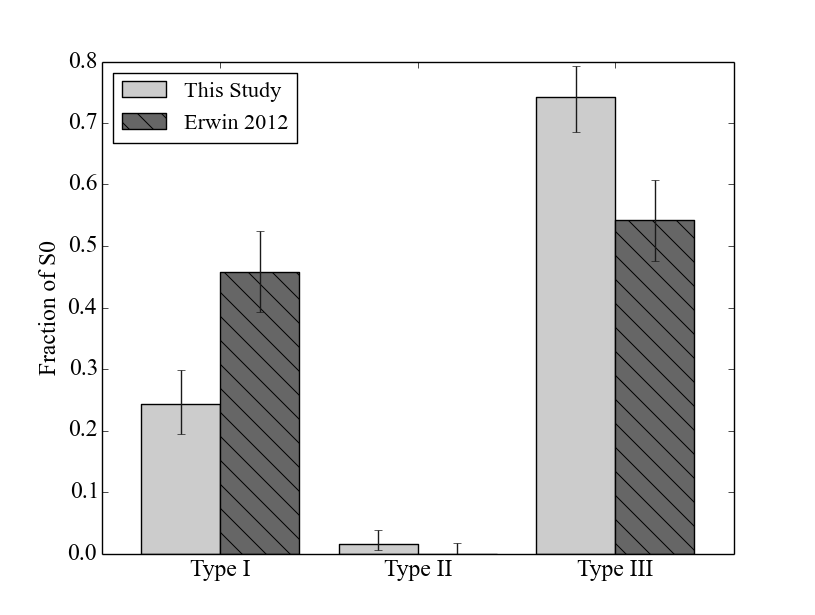
\includegraphics[width=\textwidth]{figs/total_bar_chart_truncs.png}
	\caption{Comparison of Type fraction in the Coma cluster to Virgo \citep{erwin_strong_2012}. Error bars show 68\% confidence intervals \citep{wilson_probable_1927}}
\end{figure}

\subsection{Problems with this method}
Fitting in 1D is swift and easier than a full 2D decomposition. However, neglecting most of the light of the galaxy impacts on the accuracy of the profile fitted. Any perturbation or artefact -such as a bar or flat-fielding error- included in the major axis wedge cannot be easily or safely removed. Therefore, the two major axis profiles will strongly disagree if there is a slight difference between them. Further problems arise from the combination of profiles from different cameras. 

Combining four bootstraps is effective when the individual results are already close to each other (within $\sim 1\sigma$) and a disagreeing fourth may be discarded provided the other three agree. When there is a dichotomy in parameter space larger than $\sim 2\sigma$ the resulting combination will yield a result which neither bootstrap group supports and with large errors. 

Sky detection has worked effectively in this investigation but whether our values are correct or not is untestable until there are more readings around the galaxy in addition to those at the end of the major-axis. 
\section{Conclusion}
	% !TEX root = master.tex

We have used SDSS and MegaCam \iband images to investigate truncations in S0s present in the Coma Cluster. Using a refined sample of 66 galaxies exhibiting a wide range of bulge and classical disk parameters, we have taken two 1D profiles along the the major axis for each image. The resulting four profiles were first fit with a \sersic bulge + exponential disk model with the requirement that disk dominates at large $R$. Then the truncation point was found and a truncated disk fit yielding a distribution of truncated, anti-truncated and classical exponential disks. The four profiles for each galaxy are then combined with their bootstrapped confidence intervals to give overall parameters for the galaxy.

Our main conclusions are:
\begin{itemize}
	\item 1D decomposition with truncation can be easily automated and requires little computational effort. The iterative sky finding algorithm is also effective at measuring mean sky levels at large $R$.
	\item There is a tendency for this procedure to place break radii towards the end of the profile i.e. where the sky starts to dominate. This needs to be corrected by a full component fit over the whole profile.
	\item We find strong evidence for the suppression of formation of type-II truncated galaxies in the cluster environment, in agreement with values found in the Virgo cluster \citep{erwin_strong_2012}
	\item We find that type-III anti-truncated disks are significantly more frequent than type-I single exponential disks in the cluster. 
	\item We measure that type-Is are equally frequent in both field and cluster environments. This suggests that the formation of type-IIs is heavily suppressed compared to type-IIIs.
	\item We observe brighter and more centrally compact bulges in type-IIIs than type-Is and conclude that this supports the galaxy harassment hypothesis of type-III formation
	\item We measure a weak trend of increasing type-III fraction with decreasing cluster-centric radius suggesting that type-IIIs form more frequently in high density environments
\end{itemize}

Although it is possible to characterise truncations with this method, there is significant error combining four profiles. A 2D fit and decomposition would undoubtedly render more robust and accurate results.
\bibliographystyle{mn2e(old)}
\bibliography{zotero}
\end{document}